MMS algorithm in \textit{alibi-detect} library has a online version, which also presents an interest for our case. One of the main difference of an online drift detector is that it does not accept several inputs at once and alerts whether they represent a drift or not, on the contrary --- online algorithm focuses on a single input at a time during its run. It assumes that there is a big dataset of a reference data, that can be used as an example of a "correct" distribution and processes one embedding at a time. This single input would be sent into a test window where two-sample test-statistics (MMD essentially in this case) will be calculated. As soons as the test-statistic exceeds some pre-defined threshold the drift alert is send to a user. Apart from the threshold one has to define a so-called expected run-time (ERT). This time states how many inputs the detector should process on average before it makes a detection (false positive or true positive depending on which distributions the inputs were taken from). Another hyper parameter here is hidden in a size of a test-window. Becase the larger the window is, the more chance is there to detect a very slight drift, yet with a smaller window one gets a much faster response to severe drift. 

It is usually recommened to reduce the dimensionality of the data before feeding it into the algorithm. But in this case the performance was exceptional even for high-dimensional embeddings of the UNET model. However there are also options on how to reduce the dimensionality of the data from the authors of the framework.

This algorithm was trained on the same uncorrupted training data sent through the embeddings of a nucleus UNet. Yet, test crops are fed into a detector in a consecutive way --- in case of no corruptions present it is not enough to feed only several crops from one image, as the algoritm requires more data to be fed into the detector until it makes a decision. For example, ERT of not corrupted inputs can be even up to $180$ crops until a detector alerts a false positive detection. On the contrary for corrupted inputs drift detector needs usualy $\leq 6$ crops (see Figure \ref{fig:online-ert})
\begin{figure}[H]
	\begin{center}
		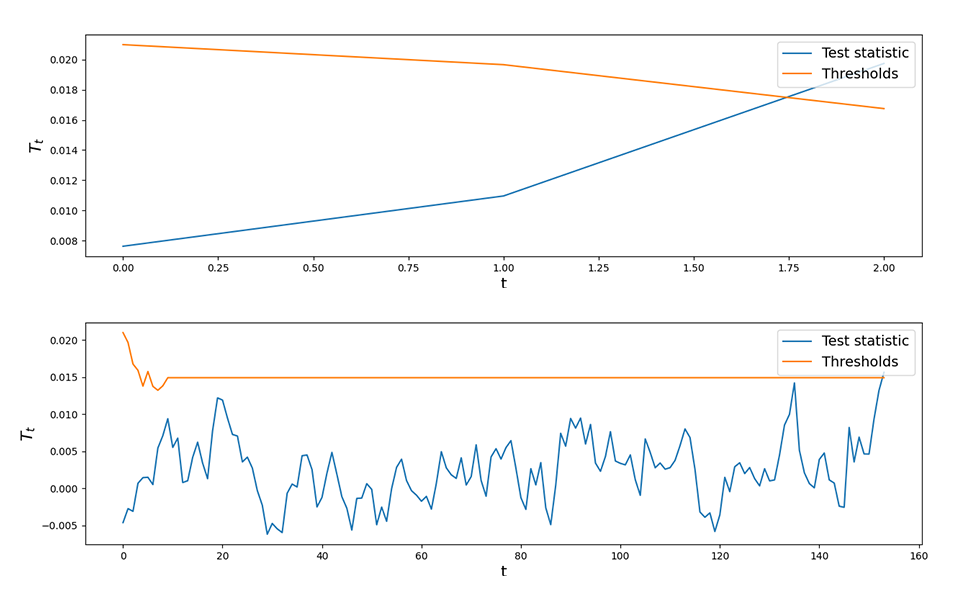
\includegraphics[width=0.6\linewidth]{bilder/drift-detection/online.png}
		\caption{Expected runtime (ERT) for corrupted and in-distribution data}\label{fig:online-ert}
	\end{center}
\end{figure}

Having such a detector one measures ERTs for not corrupted inputs, then for corrupted ones and calculated the best threshold that can separate these two. ERTs of corrupted data should be much lower than ERTs of not corrupted one. In this experiment ERTs of both classes were separable, however both located very close to the threshold: $\approx 4.59$ for corruted ones and $approx 7.1$ for not corrupted. Yet with a threshold of $6$ the accuracy scores are very high. Having a drift detector trained on not corrupted training data only, one can estimate ROC-AUC scores between two classes: not corrupted test data and the same test data but with some corruption applies to it. The results of this experiment with a defocus blur corruption of several severities are presented in Figure \ref{fig:online-auc-roc}. Already on severity 3, such detector separtes the two almost perfectly. The scores are alse presented in Table \ref{tab:severity-separability}.

\begin{figure}[htb]
	\begin{center}
		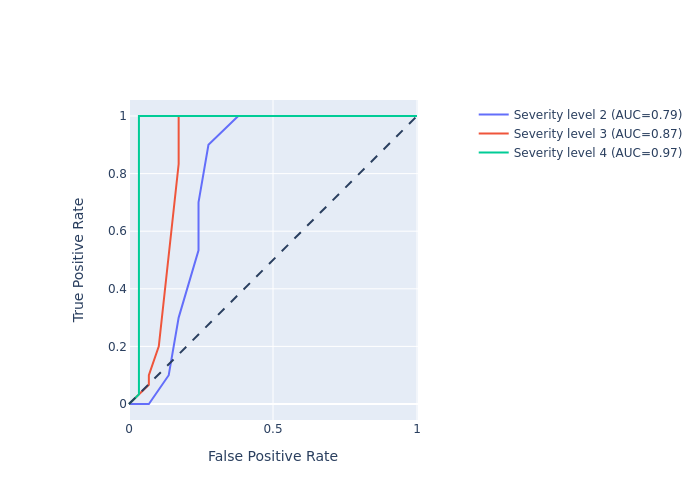
\includegraphics[width=0.8\linewidth]{bilder/drift-detection/auc_roc comparison online.png}
		\caption{AUC ROC scores for various defocus corruptions severities}\label{fig:online-auc-roc}
	\end{center}
\end{figure}

\begin{table}[htb]
    \centering
    \caption{Severity of corruptions on separability}
        \begin{adjustbox}{width=0.4\textwidth}
            \begin{tabular}{|l||*{3}{c|}}\hline
                \makebox{W}
                &\makebox[3em]{Level 2}
                &\makebox[3em]{Level 3}
                &\makebox[3em]{Level 4}
                \\\hline\hline
                Auc-Roc &0.84&0.92&0.98\\\hline
            \end{tabular}
            \label{tab:severity-separability}
        \end{adjustbox}
\end{table}

Additionally, research has been performed on the influence of the hyperparameters to an online MMD drift detector, specifically: test window size, specified ERT and presented in Tables \ref{tab:test-window-size-influence}, \ref{tab:ert-influence}. Test window size influences how fast and how sensitive the reaction of an algorithm should be and the ideal value in this case would be $10$ crops, during this time a threshold will be established. In case of ERT as a hyperparameter as long as it is big enough the score does not change very much.

\begin{table}[H]
    \centering
    \caption{Test window size influence on separability}
        \begin{adjustbox}{width=0.6\textwidth}
            \begin{tabular}{|l||*{5}{c|}}\hline
                \makebox{W}
                &\makebox[3em]{2}
                &\makebox[3em]{5}
                &\makebox[3em]{10}
                &\makebox[3em]{15}
                &\makebox[3em]{20}
                \\\hline\hline
                Auc-Roc &0.85&0.92&0.98&0.90&0.88\\\hline
            \end{tabular}
            \label{tab:test-window-size-influence}
        \end{adjustbox}
\end{table}

\begin{table}[H]
    \centering
    \caption{ERT influence on separability}
        \begin{adjustbox}{width=0.5\textwidth}
            \begin{tabular}{|l||*{4}{c|}}\hline
                \makebox{W}
                &\makebox[3em]{32}
                &\makebox[3em]{64}
                &\makebox[3em]{128}
                &\makebox[3em]{256}
                \\\hline\hline
                Auc-Roc &0.90&0.95&0.98&0.98\\\hline
            \end{tabular}
            \label{tab:ert-influence}
        \end{adjustbox}
\end{table}
